\section{Histogramme}

\subsection{Überlegungen}
Jetzt wo ich die Kreiserkennung implementiert habe, ist es mir möglich Münzen im Bild zu erkennen. Der nächste Schritt wäre es nun, die Münzen zu klassifizieren und zu unterscheiden. Doch wie klassifiziert man in openCV Bilder? Meine Idee war es, die Bilder als Histogramme zu speichern und zu vergleichen. Ein Histogramm ist eine graphische Darstellung der Häufigkeitsverteilung von Werten. In meinem Fall würde ich die Farbwerte der Münzen in einem Histogramm speichern und diese dann vergleichen.

\subsection{Die Vorlagen}
Damit ich die Münzen anhand ihrer Bildinformastionen klassifizieren kann, benötige ich zuerst Vorlagen, mit denen ich die Münzen vergleichen kann. Ich habe also Bilder von den Münzen gemacht und diese als Vorlagen gespeichert. Diese Vorlagenbilder sind die Referenzbilder, anhand derer ich die Münzen im Kamerabild auf Ähnlichkeit überprüfen möchte.

Hier hat sich vorallem die spiegelnde Oberfläche der Münzen als Problem herausgestellt. Ich musste viel mit dem Lichteinfallswinkel und der Beleuchtung spielen, um von jeder Münze ein gutes Bild zu bekommen. Auch der Abnutzungsgrad hat das Erstellen der Vorlagen erschwert. So musste ich vorallem bei den 50-20-10 Cent Münzen und bei den 5-2-1 Cent Münzen darauf achten, dass die Münzen stets eine ähnliche Optik ausweisen. Andernfalls könnte es passieren, dass die Spiegelung oder die Abnutzung als Unterschied interpretiert wird und nicht mehr die Ziffern auf den Münzen.

Meine Vorlagen sehen wie folgt aus:

\begin{figure}[ht]
    \centering
    \begin{subfigure}{0.23\textwidth}
        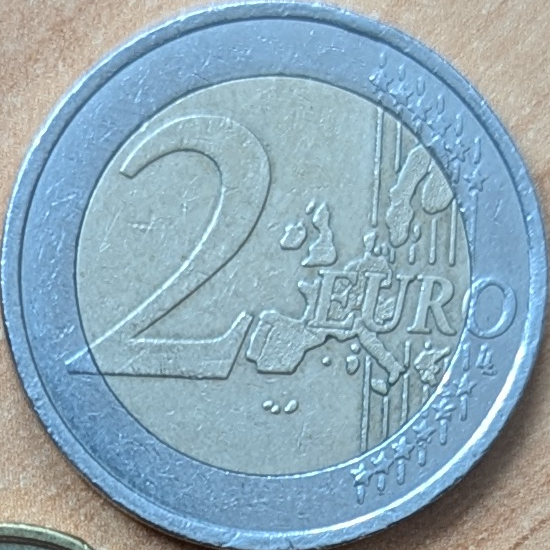
\includegraphics[width=\linewidth]{../CoinFinder/templates_2/Euro2.png}
    \end{subfigure}
    \begin{subfigure}{0.23\textwidth}
        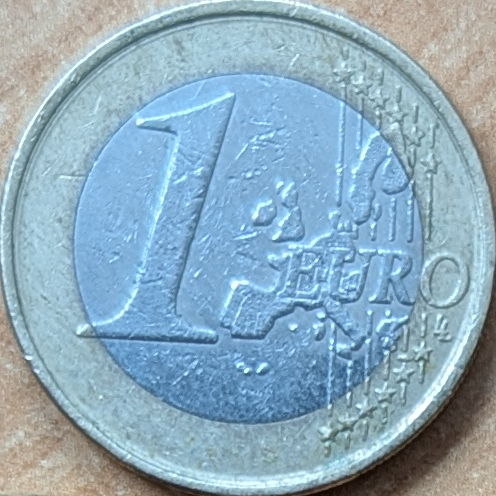
\includegraphics[width=\linewidth]{../CoinFinder/templates_2/Euro1.png}
    \end{subfigure}
    \begin{subfigure}{0.23\textwidth}
        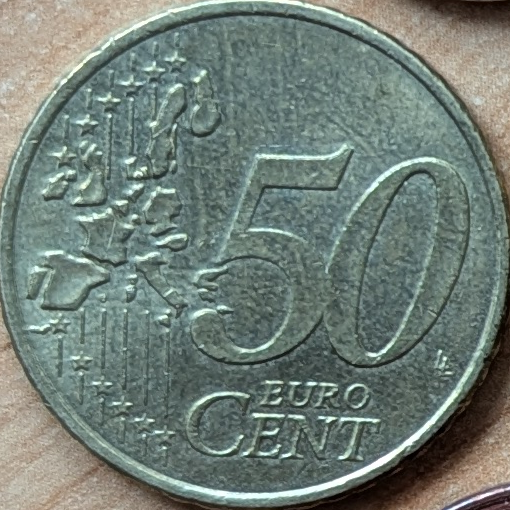
\includegraphics[width=\linewidth]{../CoinFinder/templates_2/Cent50.png}
    \end{subfigure}
    \begin{subfigure}{0.23\textwidth}
        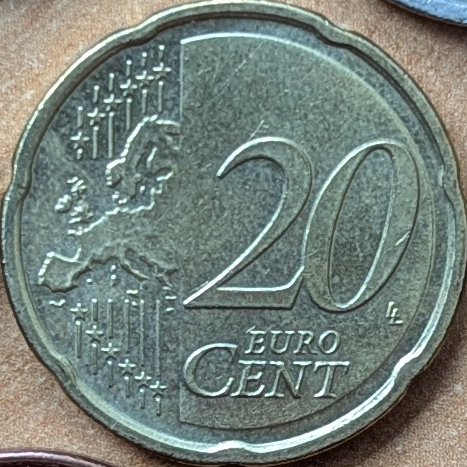
\includegraphics[width=\linewidth]{../CoinFinder/templates_2/Cent20.png}
    \end{subfigure}

    \begin{subfigure}{0.23\textwidth}
        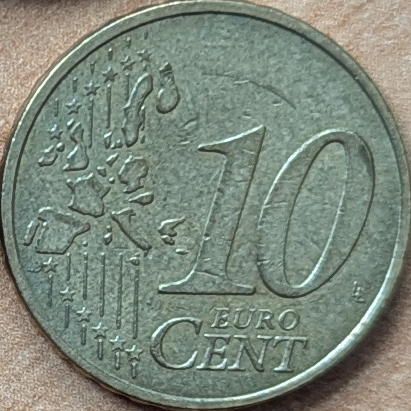
\includegraphics[width=\linewidth]{../CoinFinder/templates_2/Cent10.png}
    \end{subfigure}
    \begin{subfigure}{0.23\textwidth}
        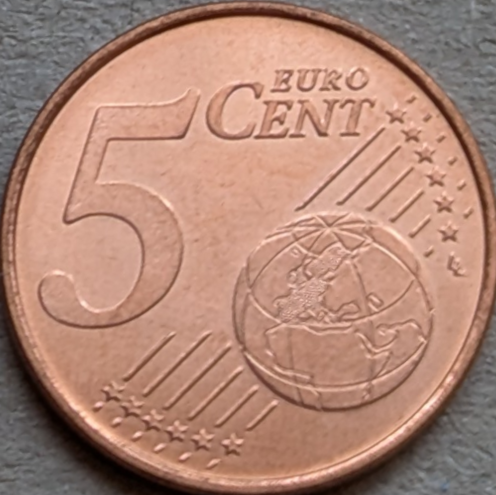
\includegraphics[width=\linewidth]{../CoinFinder/templates_2/Cent5.png}
    \end{subfigure}
    \begin{subfigure}{0.23\textwidth}
        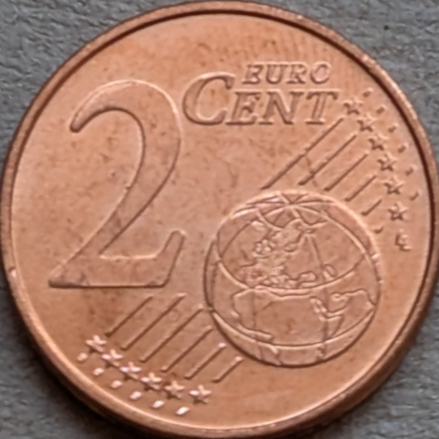
\includegraphics[width=\linewidth]{../CoinFinder/templates_2/Cent2.png}
    \end{subfigure}
    \begin{subfigure}{0.23\textwidth}
        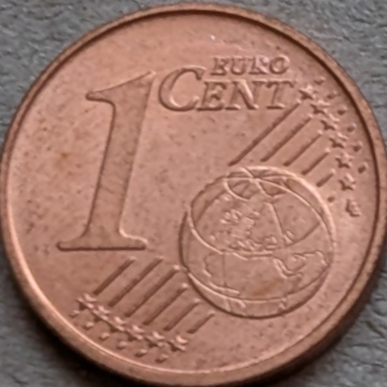
\includegraphics[width=\linewidth]{../CoinFinder/templates_2/Cent1.png}
    \end{subfigure}
\end{figure}

\subsection{Erstellung der Histogramme}

\subsection{Vergleich der Histogramme}

\subsection{Erste Ergebnisse}